\section{Task 2}
\begin{center}
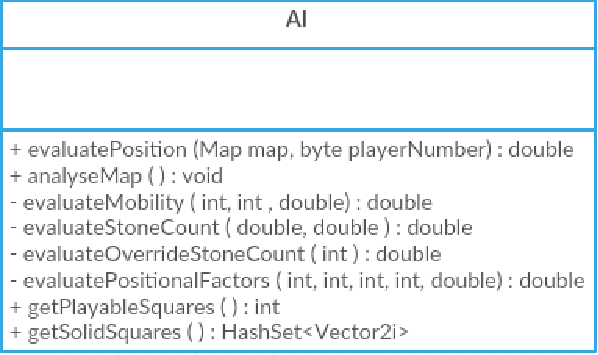
\includegraphics[scale=0.8]{AIClassdiagram.pdf}
\end{center}


Unsere Bewertungsfunktion behandelt verschiedene Aspekte des Spieles. Diese wären:
\begin{enumerate}
\item[-] Stabile Felder
\item[-] Feldkontrolle
\item[-] Mobilität (Anzahl "kostenfreier" Züge)
\item[-] Anzahl Overridesteine
\end{enumerate}
Dabei geht die Evaluationsfunktion für jede dieser Eigenschaften ähnlich vor: 
\begin{enumerate}
\item[1.] Bestimme den erwarteten Wert der Eigenschaft für die aktuelle Spielsituation
\item[2.] Multipliziere die Differenz zum realen Wert mit einem Bonusfaktor
\item[3.] Skaliere den errechneten Wert mit einer Wichtigkeitsfunktion abhängig von aktueller Spielsituation (Meistens das Stadium des Spieles)
\end{enumerate}
Die Wichtigkeitsfunktionen $$w_i:\ [0,1] \rightarrow [0,1]$$ legen demnach fest wie viel Einfluss eine Eigenschaft zu dem konkreten Zeitpunkt hat auf die Evaluation hat. Zum Beispiel ist die Anzahl der eigenen Steine (Feldkontrolle) am Anfang des Spieles nahezu unwesentlich und zum Ende hin das Einzige was zählt:
\begin{center}
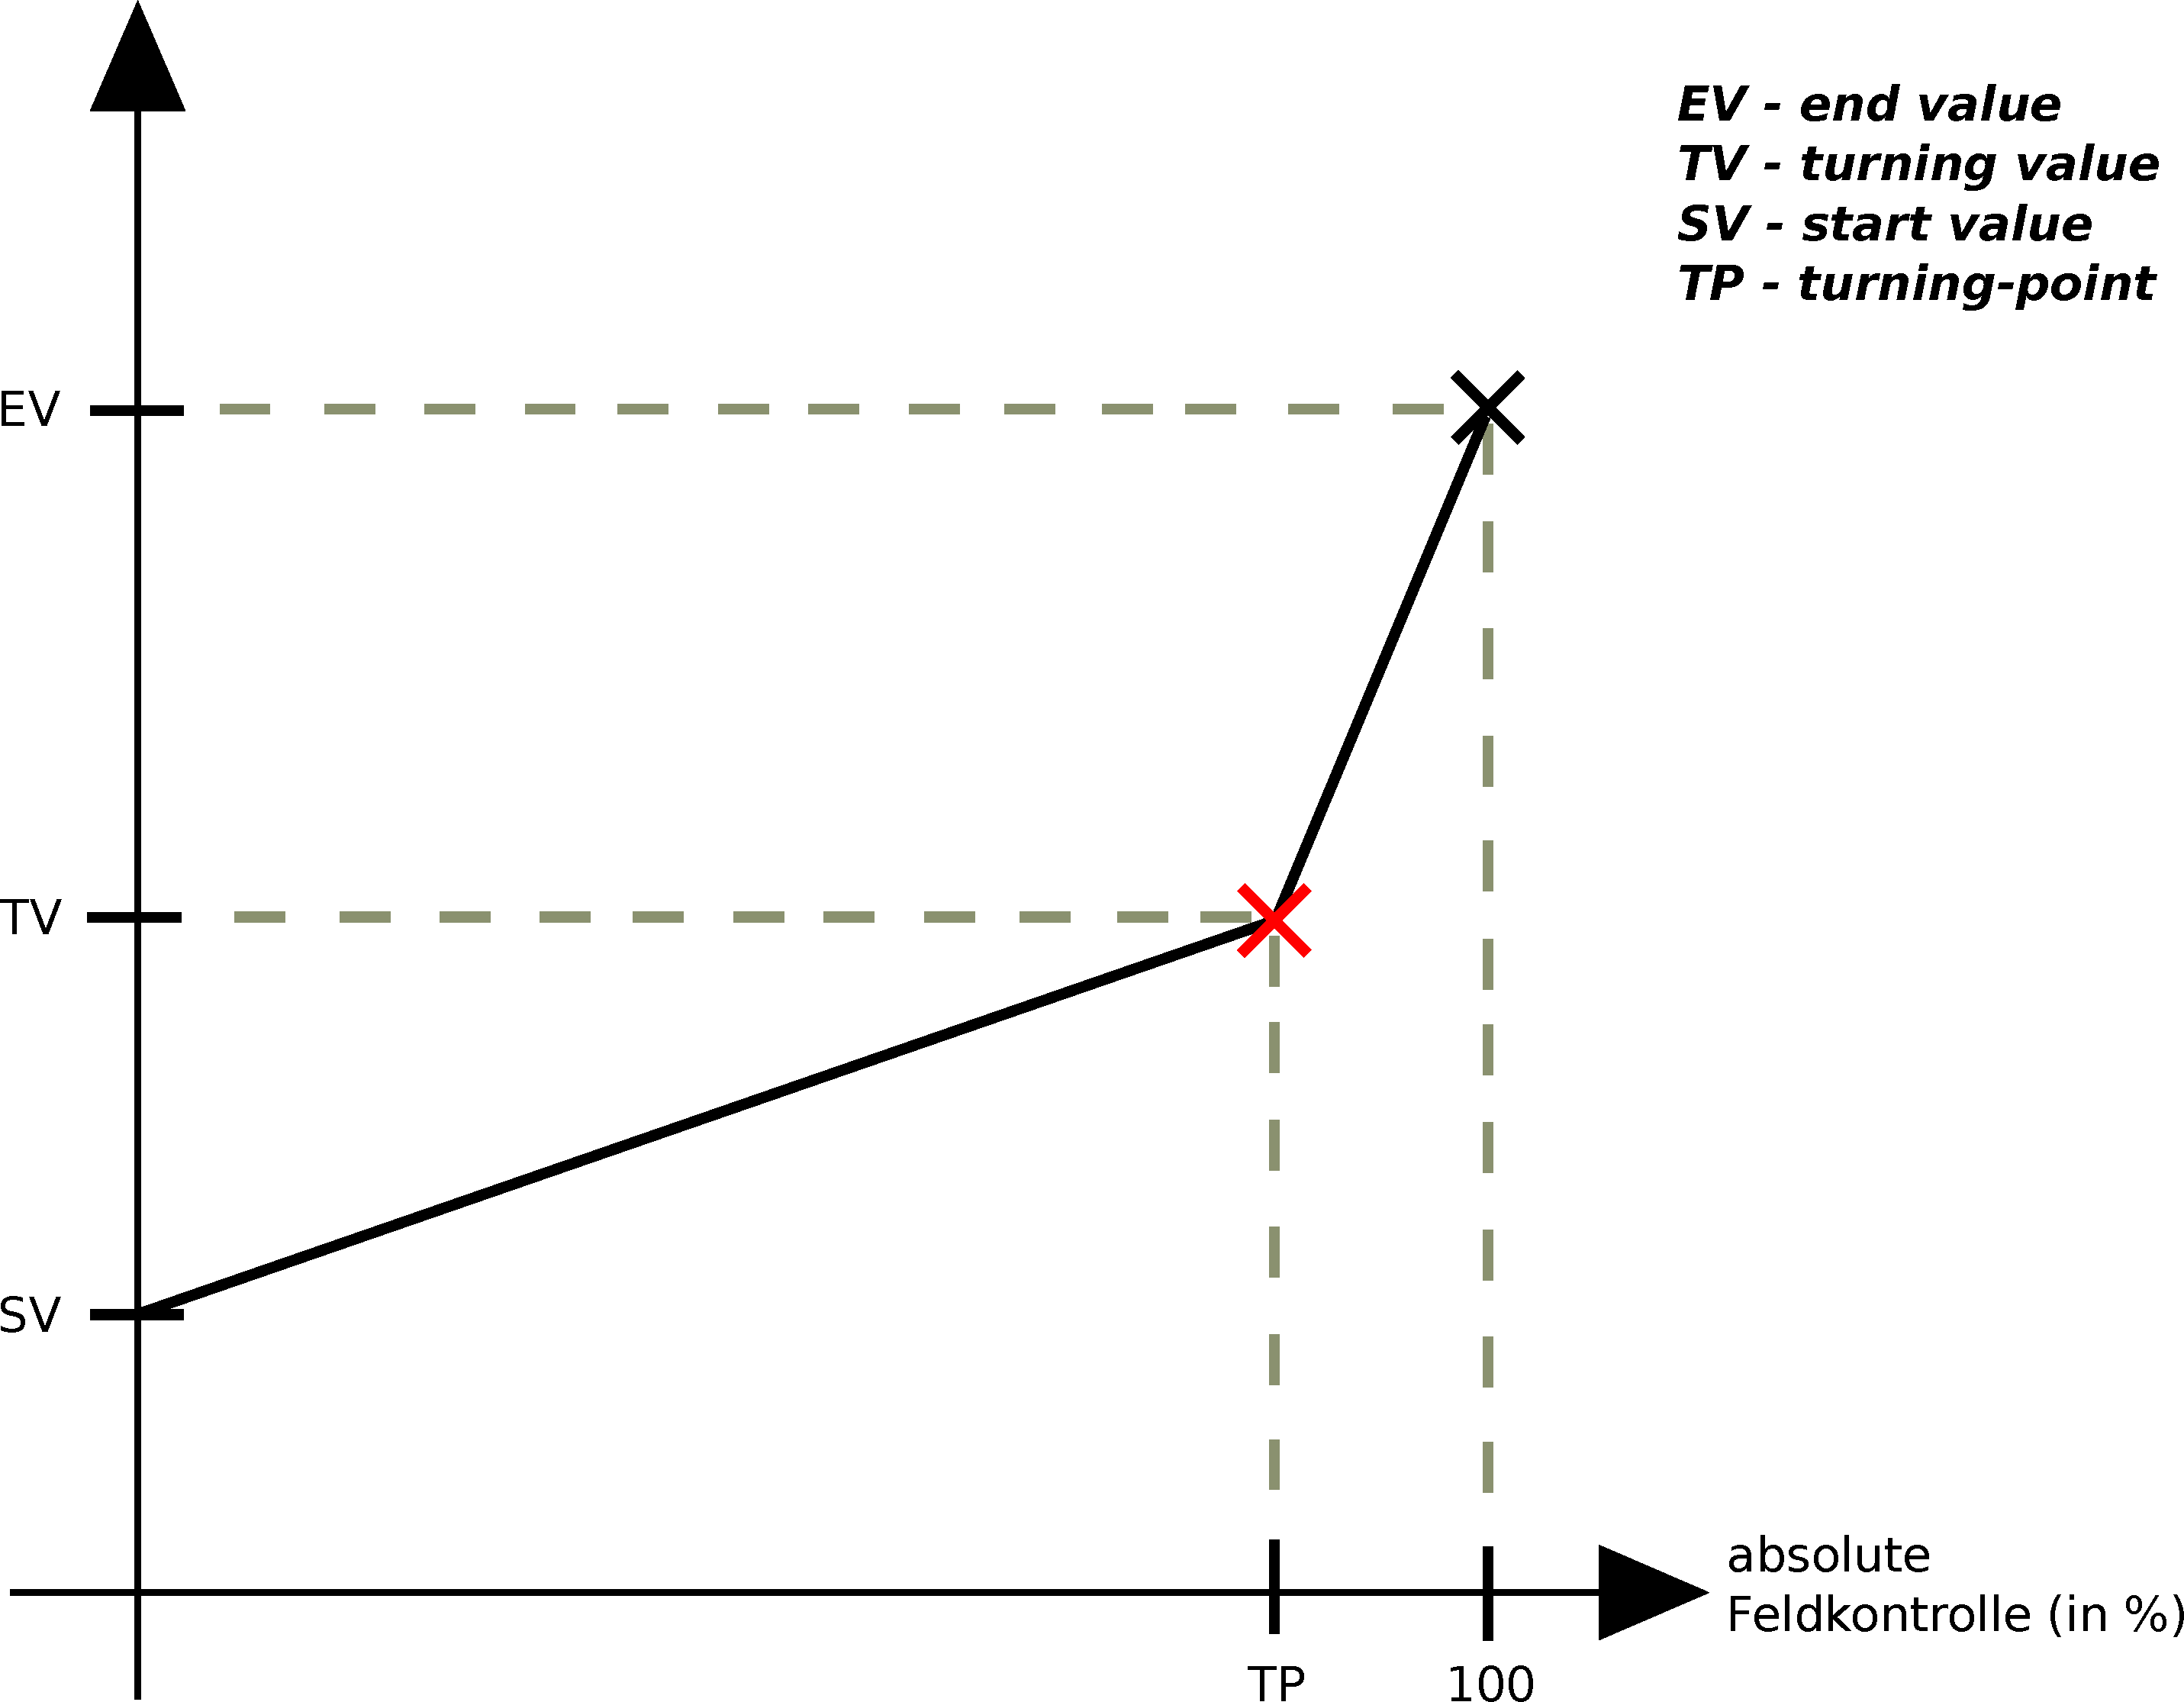
\includegraphics[scale=0.15]{ImportanceFunctionGraph.pdf}
\end{center}
Durch einfache lineare Approximation der Wichtigkeit, verlieren wir den sanften Übergang zwischen den Phasen vor und nach dem Wendepunkt. Jedoch beugen wir mögliche Überanpassung vor, welche starke Schwankungen der Funktion in manchen Bereichen zur Folge haben könnte und die Bewertung zum "Zittern" bringen würde.\\
Ähnlich sieht die Funktion aus für die stabilen Felder. Diese ist jedoch monoton fallend $SV \geq TV \geq EV$, da positionelles Spiel zum Ende hin vom konkreten Spiel verdrängt wird. Weil Mobilität stets wichtig ist, sowohl am Ende als auch am Anfang, weicht diese Wichtigkeitsfunktion ab und betrachtet die Anzahl der Spielzüge, bis man wieder selber an der Reihe ist. Die Anzahl der Overridesteine hat aus demselben Grund die Wichtigkeit konstant 1.\\\\
Die Funktionen für den erwartenden Wert sind grundsätzlich dazu da, dass sich die Stellungsbewertung nicht grundlos verbessert oder verschlechtert. So ist z.B. die Mobilität am Anfang des Spieles eingeschränkt, da noch nicht genug Steine auf dem Feld liegen. Steigt auf natürliche Art und Weise an im Laufe des Spieles und nimmt wieder ab zum Ende, da die meisten Felder belegt sind. Ignoriert man den Verlauf, verbessert sich natürlicherweise die eigene Bewertung am Anfang des Spieles (ohne etwas besonders Gutes leisten zu müssen) und verschlechtert sich zum Ende hin, auch wenn man vielleicht stark spielt. Unsere Modellierung der Mobilität ist dementsprechend:
\begin{center}
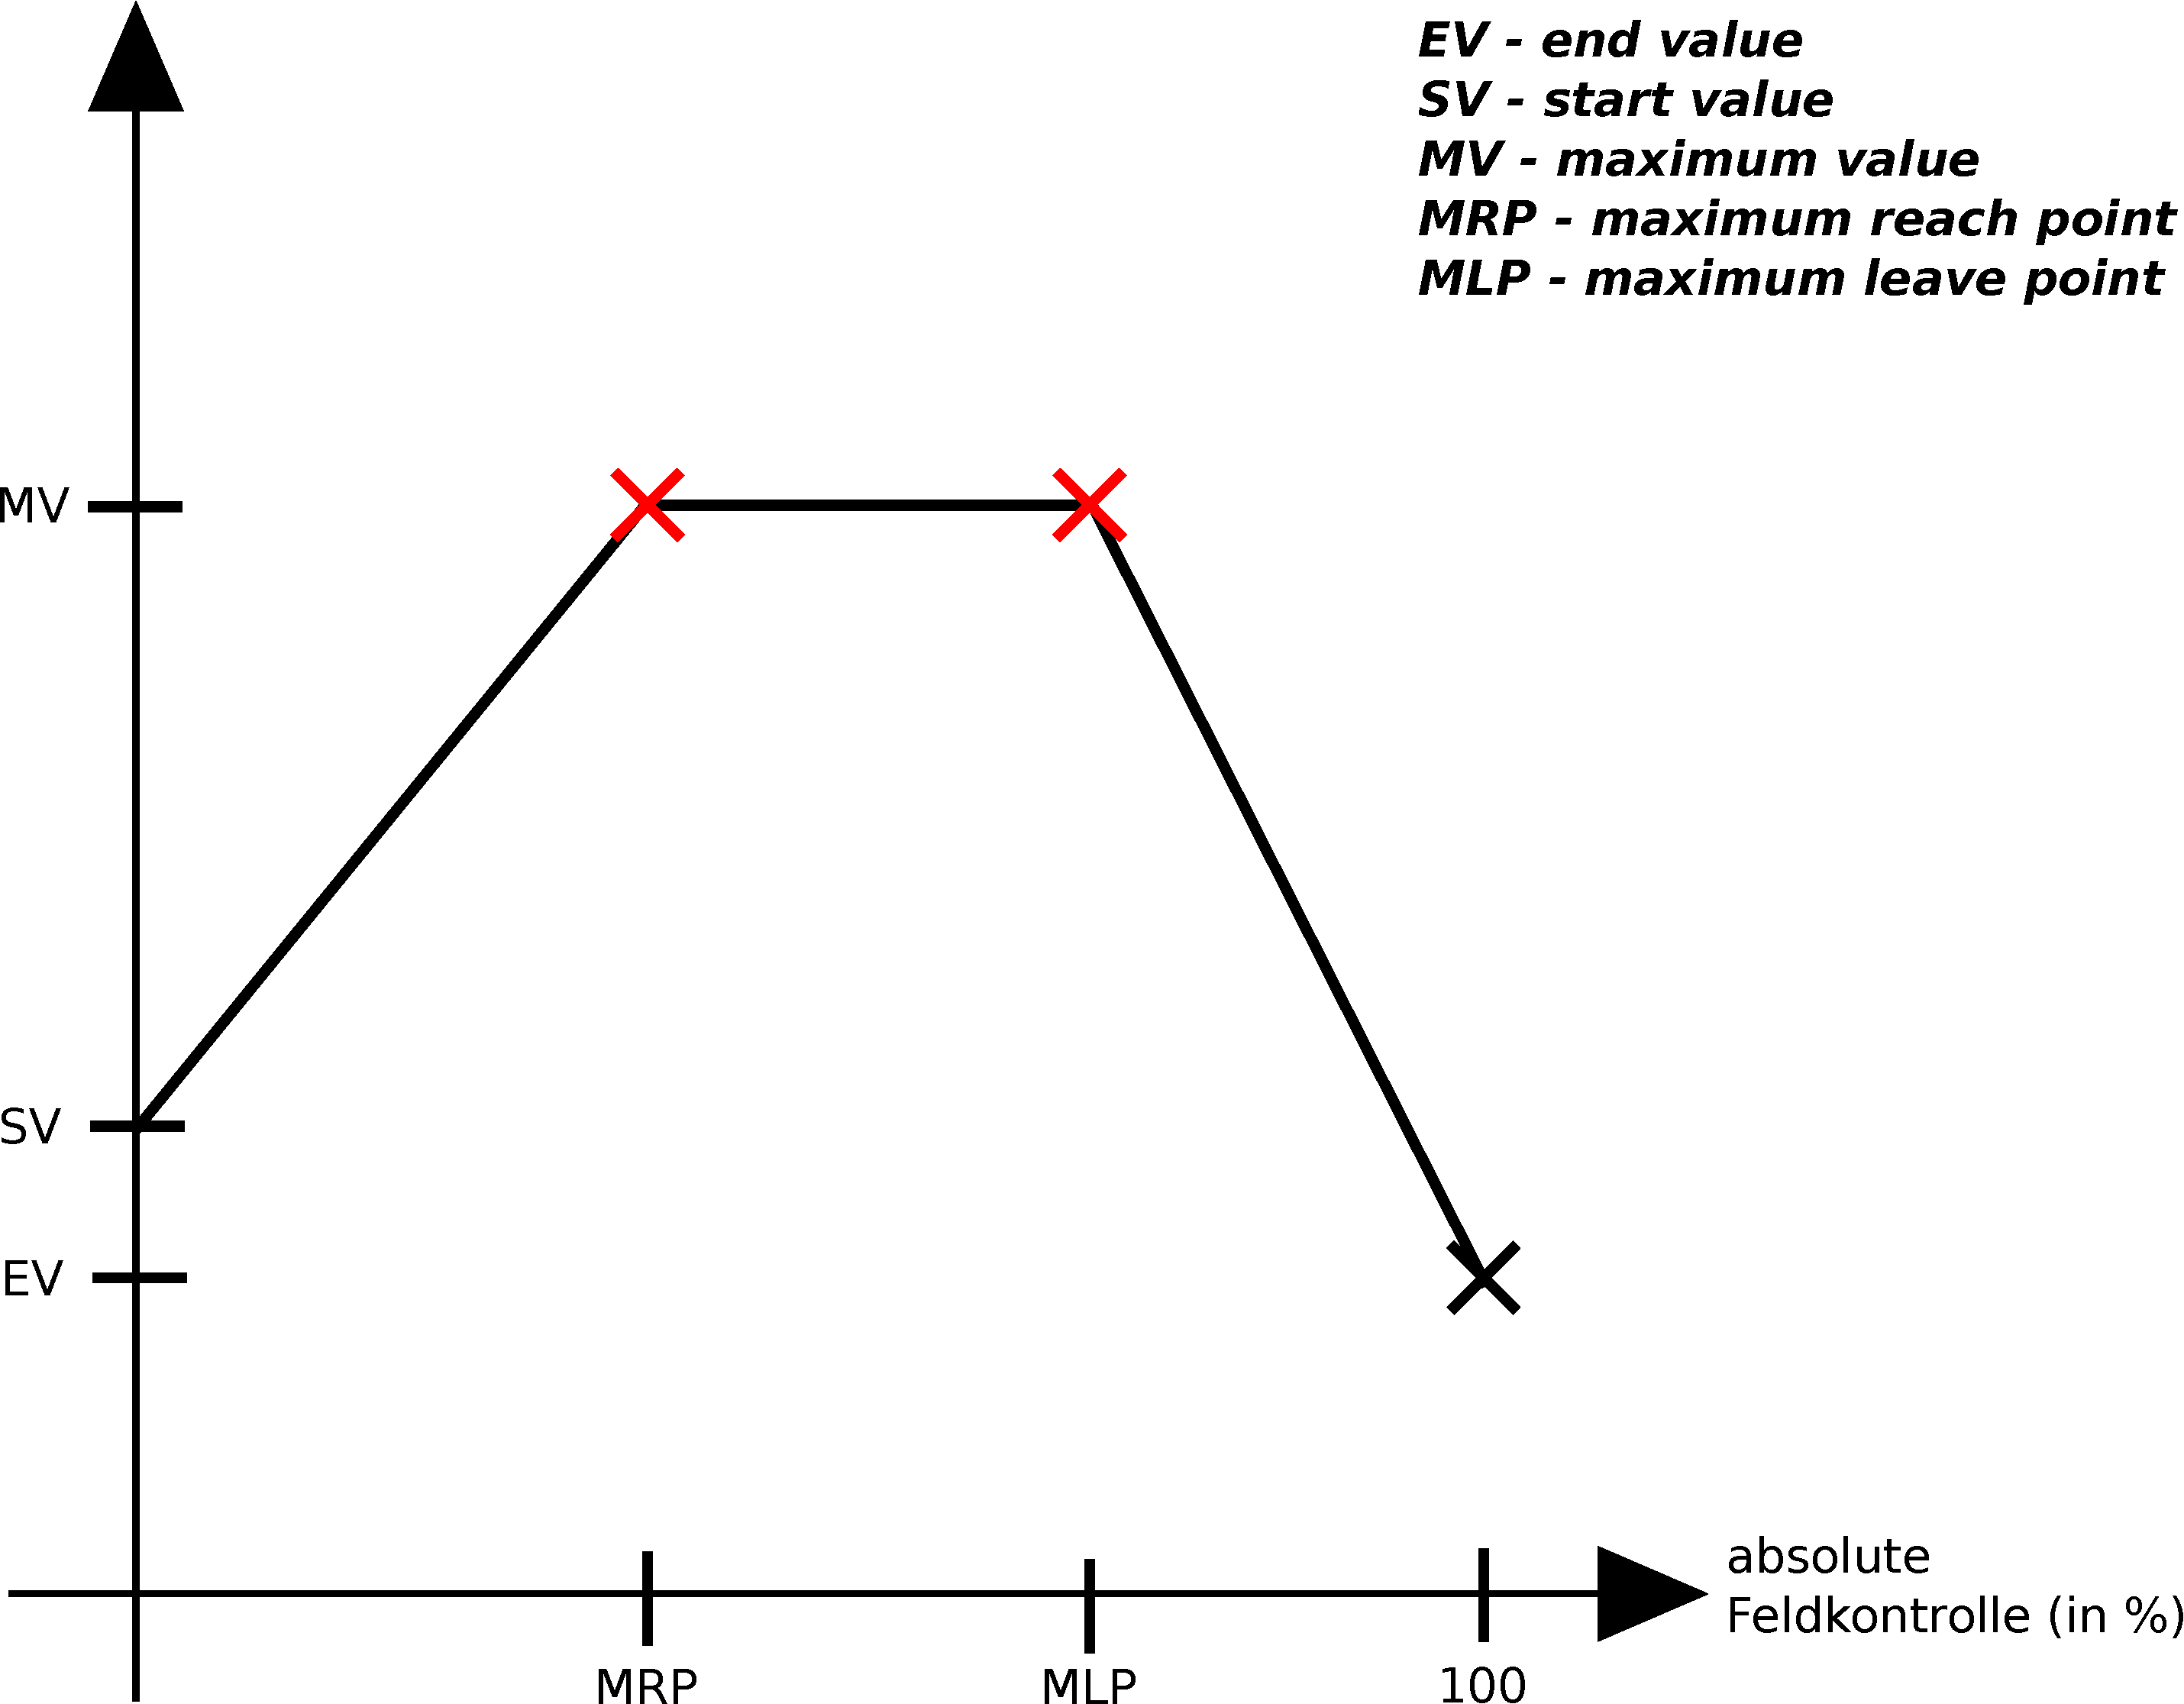
\includegraphics[scale=0.15]{ExpectedValueFunction.pdf}
\end{center}
Die Funktionen für die Anzahl der Overridesteine und stabilen Felder ist zunächst konstant 0 gelassen, aufgrund mangelnder Erfahrung und Einschätzbarkeit. Die Funktion für die eigene Feldkontrolle nimmt einen ähnlichen Verlauf wie die Wichtigkeitsfunktion.\\
Mit der hohen Parametrisierung erhoffen wir uns eine hohe und systematische Anpassbarkeit der Bewertungsfunktion. Mit steigender Spielerfahrung sollten sich gute heuristische Werte einpendeln.
\newline

\noindent
Nun haben wir auch die Methode anlayseMap, die schaut auf der ganzen Map schaut, ob es stabile Felder gibt und diese im HashSet solidSquares speichert. Die Methode iteriert über die ganze Map und schaut bei Feldern, die keine Löcher sind, ob diese stabil sind, indem man schaut ob alle 4 Richtungen blockiert sind. Ausserdem wird beim iterieren über der Map alle bespielbaren Felder mit dem Counter playableSquares gezählt.

